\documentclass{standalone}
\usepackage{tikz}
\usetikzlibrary{patterns, positioning}

\begin{document}
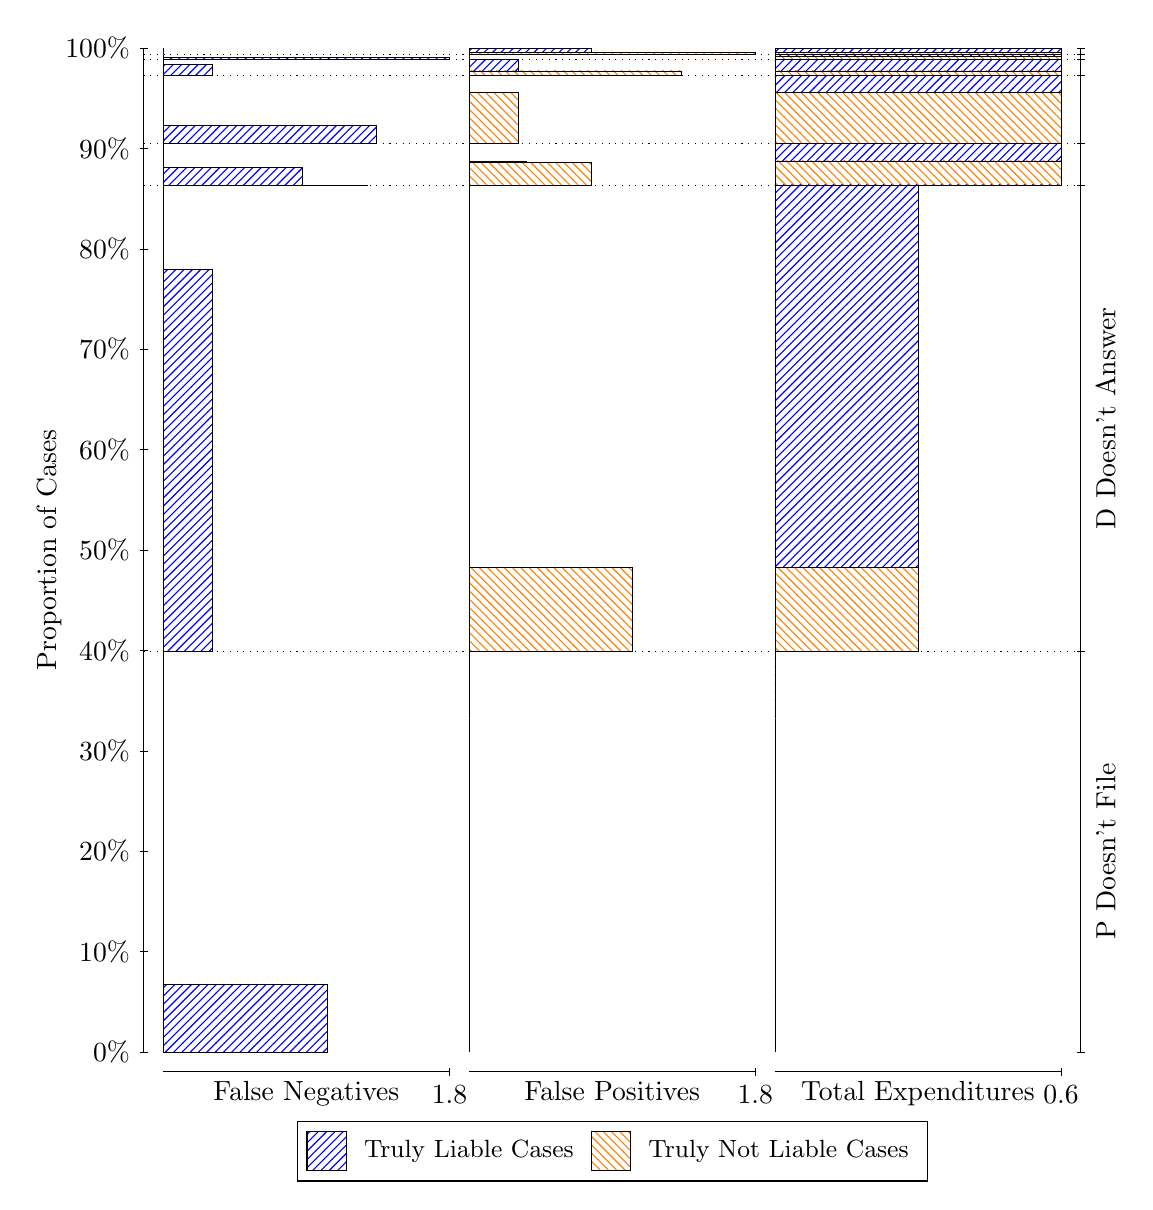
\begin{tikzpicture}
\draw[black, very thin] (1.5,1.75) -- (1.5,14.5);
\node[rotate=90, anchor=center] at (0.3, 8.125) {Proportion of Cases};
\draw[black, very thin] (1.45,1.75) -- (1.55,1.75);
\node[anchor=east] at (1.45, 1.75) {0\%};
\draw[black, very thin] (1.45,3.025) -- (1.55,3.025);
\node[anchor=east] at (1.45, 3.025) {10\%};
\draw[black, very thin] (1.45,4.3) -- (1.55,4.3);
\node[anchor=east] at (1.45, 4.3) {20\%};
\draw[black, very thin] (1.45,5.575) -- (1.55,5.575);
\node[anchor=east] at (1.45, 5.575) {30\%};
\draw[black, very thin] (1.45,6.85) -- (1.55,6.85);
\node[anchor=east] at (1.45, 6.85) {40\%};
\draw[black, very thin] (1.45,8.125) -- (1.55,8.125);
\node[anchor=east] at (1.45, 8.125) {50\%};
\draw[black, very thin] (1.45,9.4) -- (1.55,9.4);
\node[anchor=east] at (1.45, 9.4) {60\%};
\draw[black, very thin] (1.45,10.675) -- (1.55,10.675);
\node[anchor=east] at (1.45, 10.675) {70\%};
\draw[black, very thin] (1.45,11.95) -- (1.55,11.95);
\node[anchor=east] at (1.45, 11.95) {80\%};
\draw[black, very thin] (1.45,13.225) -- (1.55,13.225);
\node[anchor=east] at (1.45, 13.225) {90\%};
\draw[black, very thin] (1.45,14.5) -- (1.55,14.5);
\node[anchor=east] at (1.45, 14.5) {100\%};

\draw[black, very thin] (13.4,1.75) -- (13.4,14.5);
\draw[black, very thin] (13.35,1.75) -- (13.45,1.75);
\node[anchor=west] at (13.35, 1.75) {};
\draw[black, very thin] (13.35,6.8406) -- (13.45,6.8406);
\node[anchor=west] at (13.35, 6.8406) {};
\draw[black, very thin] (13.35,12.753) -- (13.45,12.753);
\node[anchor=west] at (13.35, 12.753) {};
\draw[black, very thin] (13.35,13.293) -- (13.45,13.293);
\node[anchor=west] at (13.35, 13.293) {};
\draw[black, very thin] (13.35,14.151) -- (13.45,14.151);
\node[anchor=west] at (13.35, 14.151) {};
\draw[black, very thin] (13.35,14.351) -- (13.45,14.351);
\node[anchor=west] at (13.35, 14.351) {};
\draw[black, very thin] (13.35,14.42) -- (13.45,14.42);
\node[anchor=west] at (13.35, 14.42) {};
\draw[black, very thin] (13.35,14.5) -- (13.45,14.5);
\node[anchor=west] at (13.35, 14.5) {};

\draw[black, very thin, pattern color=blue, pattern=north east lines] (1.75,1.75) rectangle (3.8262,2.6054);
\draw[black, very thin, pattern color=orange, pattern=north west lines] (1.75,2.6054) rectangle (1.75,6.8406);
\draw[black, very thin, pattern color=blue, pattern=north east lines] (1.75,6.8406) rectangle (2.3729,11.69);
\draw[black, very thin, pattern color=orange, pattern=north west lines] (1.75,11.69) rectangle (1.75,12.753);
\draw[black, very thin, pattern color=blue, pattern=north east lines] (1.75,12.753) rectangle (4.3452,12.757);
\draw[black, very thin, pattern color=blue, pattern=north east lines] (1.75,12.757) rectangle (3.93,12.759);
\draw[black, very thin, pattern color=blue, pattern=north east lines] (1.75,12.759) rectangle (3.5148,12.982);
\draw[black, very thin, pattern color=orange, pattern=north west lines] (1.75,12.982) rectangle (1.75,13.293);
\draw[black, very thin, pattern color=blue, pattern=north east lines] (1.75,13.293) rectangle (4.449,13.513);
\draw[black, very thin, pattern color=orange, pattern=north west lines] (1.75,13.513) rectangle (1.75,14.151);
\draw[black, very thin, pattern color=blue, pattern=north east lines] (1.75,14.151) rectangle (2.3729,14.292);
\draw[black, very thin, pattern color=orange, pattern=north west lines] (1.75,14.292) rectangle (1.75,14.351);
\draw[black, very thin, pattern color=blue, pattern=north east lines] (1.75,14.351) rectangle (5.3833,14.378);
\draw[black, very thin, pattern color=orange, pattern=north west lines] (1.75,14.378) rectangle (1.75,14.42);
\draw[black, very thin, pattern color=orange, pattern=north west lines] (1.75,14.42) rectangle (1.75,14.446);
\draw[black, very thin, pattern color=blue, pattern=north east lines] (1.75,14.446) rectangle (1.75,14.5);
\draw[black, very thin, pattern color=orange, pattern=north west lines] (5.6333,1.75) rectangle (5.6333,5.9852);
\draw[black, very thin, pattern color=blue, pattern=north east lines] (5.6333,5.9852) rectangle (5.6333,6.8406);
\draw[black, very thin, pattern color=orange, pattern=north west lines] (5.6333,6.8406) rectangle (7.7095,7.9037);
\draw[black, very thin, pattern color=blue, pattern=north east lines] (5.6333,7.9037) rectangle (5.6333,12.753);
\draw[black, very thin, pattern color=orange, pattern=north west lines] (5.6333,12.753) rectangle (7.1905,13.045);
\draw[black, very thin, pattern color=orange, pattern=north west lines] (5.6333,13.045) rectangle (6.7752,13.05);
\draw[black, very thin, pattern color=orange, pattern=north west lines] (5.6333,13.05) rectangle (6.36,13.064);
\draw[black, very thin, pattern color=blue, pattern=north east lines] (5.6333,13.064) rectangle (5.6333,13.293);
\draw[black, very thin, pattern color=orange, pattern=north west lines] (5.6333,13.293) rectangle (6.2562,13.932);
\draw[black, very thin, pattern color=blue, pattern=north east lines] (5.6333,13.932) rectangle (5.6333,14.151);
\draw[black, very thin, pattern color=orange, pattern=north west lines] (5.6333,14.151) rectangle (8.3324,14.21);
\draw[black, very thin, pattern color=blue, pattern=north east lines] (5.6333,14.21) rectangle (6.2562,14.351);
\draw[black, very thin, pattern color=orange, pattern=north west lines] (5.6333,14.351) rectangle (5.6333,14.393);
\draw[black, very thin, pattern color=blue, pattern=north east lines] (5.6333,14.393) rectangle (5.6333,14.42);
\draw[black, very thin, pattern color=orange, pattern=north west lines] (5.6333,14.42) rectangle (9.2667,14.446);
\draw[black, very thin, pattern color=blue, pattern=north east lines] (5.6333,14.446) rectangle (7.1905,14.5);
\draw[black, very thin, pattern color=orange, pattern=north west lines] (9.5167,1.75) rectangle (9.5167,5.9852);
\draw[black, very thin, pattern color=blue, pattern=north east lines] (9.5167,5.9852) rectangle (9.5167,6.8406);
\draw[black, very thin, pattern color=orange, pattern=north west lines] (9.5167,6.8406) rectangle (11.333,7.9037);
\draw[black, very thin, pattern color=blue, pattern=north east lines] (9.5167,7.9037) rectangle (11.333,12.753);
\draw[black, very thin, pattern color=orange, pattern=north west lines] (9.5167,12.753) rectangle (13.15,12.759);
\draw[black, very thin, pattern color=blue, pattern=north east lines] (9.5167,12.759) rectangle (13.15,12.761);
\draw[black, very thin, pattern color=orange, pattern=north west lines] (9.5167,12.761) rectangle (13.15,13.067);
\draw[black, very thin, pattern color=blue, pattern=north east lines] (9.5167,13.067) rectangle (13.15,13.293);
\draw[black, very thin, pattern color=orange, pattern=north west lines] (9.5167,13.293) rectangle (13.15,13.932);
\draw[black, very thin, pattern color=blue, pattern=north east lines] (9.5167,13.932) rectangle (13.15,14.151);
\draw[black, very thin, pattern color=orange, pattern=north west lines] (9.5167,14.151) rectangle (13.15,14.21);
\draw[black, very thin, pattern color=blue, pattern=north east lines] (9.5167,14.21) rectangle (13.15,14.351);
\draw[black, very thin, pattern color=orange, pattern=north west lines] (9.5167,14.351) rectangle (13.15,14.393);
\draw[black, very thin, pattern color=blue, pattern=north east lines] (9.5167,14.393) rectangle (13.15,14.42);
\draw[black, very thin, pattern color=orange, pattern=north west lines] (9.5167,14.42) rectangle (13.15,14.446);
\draw[black, very thin, pattern color=blue, pattern=north east lines] (9.5167,14.446) rectangle (13.15,14.5);
\draw[black, dotted] (1.5,6.8406) -- (13.4,6.8406);
\draw[black, dotted] (1.5,12.753) -- (13.4,12.753);
\draw[black, dotted] (1.5,13.293) -- (13.4,13.293);
\draw[black, dotted] (1.5,14.151) -- (13.4,14.151);
\draw[black, dotted] (1.5,14.351) -- (13.4,14.351);
\draw[black, dotted] (1.5,14.42) -- (13.4,14.42);
\draw[black, very thin] (1.75,1.5) -- (5.3833,1.5);
\node[anchor=north] at (3.5667, 1.5) {False Negatives};
\draw[black, very thin] (5.3833,1.45) -- (5.3833,1.55);
\node[anchor=north] at (5.3833, 1.45) {1.8};

\draw[black, very thin] (5.6333,1.5) -- (9.2667,1.5);
\node[anchor=north] at (7.45, 1.5) {False Positives};
\draw[black, very thin] (9.2667,1.45) -- (9.2667,1.55);
\node[anchor=north] at (9.2667, 1.45) {1.8};

\draw[black, very thin] (9.5167,1.5) -- (13.15,1.5);
\node[anchor=north] at (11.333, 1.5) {Total Expenditures};
\draw[black, very thin] (13.15,1.45) -- (13.15,1.55);
\node[anchor=north] at (13.15, 1.45) {0.6};

\node[black, centered, rotate=90] at (13.72, 4.2953) {P Doesn't File};
\node[black, centered, rotate=90] at (13.72, 9.7969) {D Doesn't Answer};






\draw (7.449999999999999,1.5) node[draw=none] (baseCoordinate) {};
\begin{scope}[align=center]
        \matrix[scale=0.5, draw=black, below=0.5cm of baseCoordinate, nodes={draw}, column sep=0.1cm]{
            \node[rectangle, draw, minimum width=0.5cm, minimum height=0.5cm, pattern=north east lines, pattern color=blue] {}; &
            \node[draw=none, font=\small] (B) {Truly Liable Cases}; &
            \node[rectangle, draw, minimum width=0.5cm, minimum height=0.5cm, pattern=north west lines, pattern color=orange] {}; &
            \node[draw=none, font=\small] (B) {Truly Not Liable Cases}; \\
            };
\end{scope}

\end{tikzpicture}
\end{document}